% -*- coding: utf-8 -*-

\chapter{Localización y mapas}

El sistema de localización realizado no incorpora la construcción simultánea de mapas de los tipos descritos en el capítulo de Estado del Arte sino que elabora y luego va actualizando un mapa de puntos a partir de las observaciones correspondientes a las medidas del láser. Son los puntos que ya forman parte del mapa los que se utilizan para la localización en cada instante. Se trata de un método de \emph{máxima probabilidad incremental} basado en el filtro extendido de Kalman.

\section{Aplicación del EKF a la localización del robot: descripción del algoritmo}

En el problema que se trata, el estado queda definido por la posición del robot, $[x_{R},y_{R},\theta_{R}]^{T}$. Las medidas de la odometría (incrementales, luego referenciadas al sistema de coordenadas local del robot) constituyen las entradas al sistema, $\vec{u}=\pmatrix{u_{x}\cr u_{y}\cr \theta_{u}}$, en cada instante (se suprimen sus subíndices de tiempo para simplificar la notación; siempre se utilizan las últimas medidas disponibles). De esta forma, el modelo de estado identificable con  \ref{eq:estado_nolineal} es:

 \begin{equation}\label{estado_robot}
    \vec{x}_{R_{k}} = \vec{x}_{R_{k-1}}\oplus \vec{u} +\vec{\rho}_{\rho},
 \end{equation}

 siendo $\oplus$ el operador composición de transformaciones relativas.

\textbf{Etapa de predicción}
De acuerdo con esto, la predicción del estado dada por \ref{eq:x_predictionEKF} será:
\begin{equation}\label{eq:x_prediction_robot}
     \pmatrix{\tilde{x}_{R_{k}}\cr \tilde{y}_{R_{k}}\cr \tilde{\theta}_{R_{k}}} =
     \pmatrix{\hat{x}_{R_{k-1}}+u_{x}cos\hat{\theta}_{R_{k-1}}-u_{y}sen\hat{\theta}_{R_{k-1}}\cr \hat{y}_{R_{k-1}}+u_{x}sen\hat{\theta}_{R_{k-1}}+u_{y}cos\hat{\theta}_{R_{k-1}} \cr \hat{\theta}_{R_{k-1}}+\theta_{u}}
\end{equation}

Para la matriz de covarianza de $x_{k}$ la ecuación \ref{eq:P_predictionEKF} varía ligeramente ya que lo que se conoce no es la matriz de covarianza del proceso conjunto, $Q_{p}$,sino la covarianza del ruido presente en la odometría $\vec{u}$. Si esta variable gaussiana se representa por $\vec{u}_{k}\sim N(\hat{\vec{u}}_{k},Q)$ (tomaremos un valor constante para la covarianza del ruido de los encoders) la predicción de la covarianza del estado será:

\begin{equation}\label{eq:P_prediction_robot}
    \tilde{P}_{k} = F_{x}\hat{P}_{k-1}F_{x}^{T}+F_{u}QF_{u}^{T},
\end{equation}

donde $F_{x} = \frac{\delta f}{\delta x}\mid _{\tilde{x}_k}$ y $F_{u} = \frac{\delta f}{\delta u}\mid _{\tilde{x}_k}$ (se emplea la mejor estimación del estado disponible hasta el momento).

El resultado del cálculo de estas matrices jacobianas se incluye en el Anexo A.

El algoritmo se inicia partiendo de $\hat{x}_{0} = 0, \hat{P}_{0} = 0$.

\textbf{Etapa de corrección}
Las medidas, observaciones realizadas por el láser, se relacionan con el estado de forma implícita mediante composición con él y comparación con los puntos del mapa que se utilice. Como puede verse en la figura \ref{fg:medidas}, la expresión que liga idealmente el estado con la observación i por medio del punto del mapa j asociado a ella será:

\begin{equation}\label{eq:medidas}
    \vec{h_{ij}} = \vec{x_{R}} \oplus \vec{o_{i}} - \vec{l_{j}} = \vec{0},
\end{equation}

Aplicando la definición del operador $\oplus$ (Anexo A), \ref{eq:medidas} queda:

\begin{equation}\label{eq:hij}
    \vec{h_{ij}} = \pmatrix{-x_{lj}+x_{R}+o_{ix}cos\theta_{R}-o_{iy}sen\theta_{R}\cr -y_{lj}+y_{R}+o_{ix}sen\theta_{R}+o_{iy}cos\theta_{R}} = \vec{0},
\end{equation}

como puede obtenerse a partir de la figura \ref{fg:medidas}.

\begin{figure}[h]
  % Requires \usepackage{graphicx}
  \centering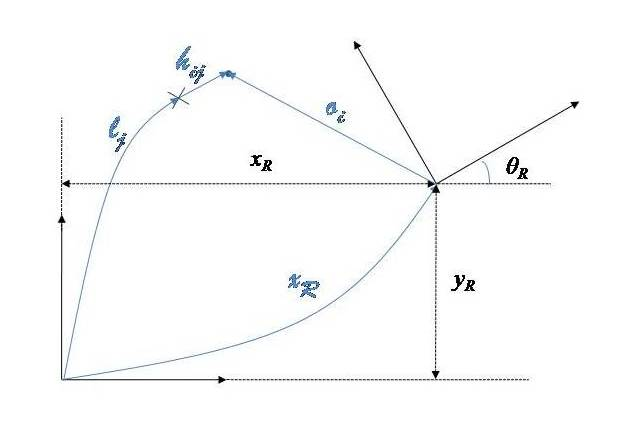
\includegraphics[scale=0.7]{dibujo1}\\
  \caption{Representación de la ecuación de medida del robot}\label{fg:medidas}
\end{figure}


Denotando $H_{x_{ij_{k}}} = \frac{\delta \vec{h_{ij}}}{\delta \vec{x}}\mid _{\tilde{x}_k,z_{k}}$ y $H_{z_{ij_{k}}} = \frac{\delta \vec{h_{ij}}}{\delta \vec{z}}\mid _{\tilde{x}_k,z_{k}}$ para cada iteración k, la matriz de covarianza de una innovación individual viene dada por \ref{eq:SEKF_im}:

\begin{equation}\label{eq:Sij_robot}
    S_{ij_{k}} = H_{x_{ij_{k}}}\tilde{P}_{k}H_{x_{ij_{k}}}^{T}+H_{z_{ij_{k}}}RH_{z_{ij_{k}}}^{T}
\end{equation}

Como puede verse en \ref{eq:Sij_robot}, la covarianza en las medidas del láser también se tomará como constante.

El cálculo de la distancia de Mahalanobis de la innovación $h_{ij_{k}}$ mediante esta matriz $S_{k}$ permitirá realizar la asociación de cada observación \emph{i} al punto del mapa \emph{j} para el cual esa distancia sea mínima. Si dicha asociación supera el test de Mahalanobis, se tendrá en cuenta para corregir la posición del robot, en caso contrario se podrá añadir la observación como nuevo punto del mapa.De entre todas las matrices $h_{ij}, H_{x_{ij}} y H_{z{ij}}$ calculadas para cada observación asociada a un punto del mapa se utilizarán únicamente las correspondientes a dicho punto. Estas matrices se denotarán $hi_{min}, Hxi_{min}, Hzi_{min}$.

Según se van asociando observaciones, se tienen más medidas que utilizar. Por ello, las dimensiones de las matrices $h, H_{x}, H_{z} y R$ irán creciendo al irse añadiendo datos. Su tamaño final en cada iteración determinará las dimensiones de S y K.

Para un número t de observaciones asociadas en la iteración k, se tiene:

\begin{center}
dim($h_{k}$)= $2t \times 1$,

dim($H_{x_{k}}$) = $2t \times 3$,

dim($H_{z_{k}}$) = $2t \times 2t$,

dim($R_{k}$) = $2t \times 2t$
\end{center}


Con lo que la matriz S global calculada a partir de ellas por medio de \ref{eq:SEKF_im} será:

\begin{equation}\label{eq:S_robot}
    S_{k} = H_{x_{k}}\tilde{P}_{k}H_{x_{k}}^{T}+H_{z_{k}}RH_{z_{k}}^{T}
\end{equation}

y tendrá dimensión ($2t \times 2t$).

La matriz de Kalman del sistema, viene dada por \ref{eq:KEKF_im}:

\begin{equation}\label{eq:K_robot}
    K_{k} = \tilde{P}_{k}H_{x_{k}}^{T}S_{k}^{-1}
\end{equation}

por lo que su tamaño será ($3 \times 2t$).

Finalmente, los valores corregidos de la posición del robot y su covarianza se obtienen a partir de la predicción de acuerdo con \ref{eq:x_estimationIm} y \ref{eq:P_estimationEKF_im}:

\begin{equation}\label{eq:x_robot}
    \hat{x}_{k} = \tilde{x}_{k} - K_{k}h_{k}
\end{equation}

\begin{equation}\label{eq:P_robot}
    \hat{P}_{k} = (I-K_{k}H_{x_{k}})\tilde{P}_{k}
\end{equation}


\section{Consideraciones sobre el coste computacional de la localización} \label{computacional}

El coste computacional de la etapa de corrección del algoritmo puede llevar a tiempos de procesamiento altos, lo que conduce a un comportamiento del sistema poco eficaz. A continuación se realiza un análisis del mismo y se identifican las principales fuentes de retardo en el cómputo de la posición corregida.

Para $n$ puntos en el mapa y $t$ observaciones adquiridas por el láser, el coste computacional de la etapa de asociación de datos es de orden $O(nt)$.

El cálculo de la matriz de ganancia de Kalman se realiza mediante \ref{eq:K_robot}. Al tener la matriz $\tilde{P}_{k}H_{x_{k}}^{T}$ dimensión ($3 \times 2t$) y $S$ dimensión ($2t \times 2t$), el coste computacional para hallar la matriz $K$ será $O(t^{3})$.

Sin variar el coste computacional, puede verse que una forma sencilla de reducir el tiempo de cálculo consiste en reducir el número de observaciones a tener en cuenta. Las observaciones que se encuentran muy alejadas del robot (distancias superiores a 6m) directamente son ignoradas. El láser proporciona medidas a intervalos de 1º (181 medidas en total) o bien a intervalos de 0.5º (361 medidas en total). Utilizando sólo una de cada dos observaciones asociadas se logra una reducción de tiempo considerable sin que se aprecien pérdidas en los resultados de la localización.

Las operaciones que inicialmente consumían más tiempo en el procesamiento de las observaciones eran la declaración de las matrices $h_{ij}, H_{x_{ij}} y H_{z{ij}}$ para todas las innovaciones y el ir ampliando las matrices $h, H_{x}, H_{z}$ y $R$ por filas o por columnas a medida que se asociaban más datos, con la consiguiente reserva de memoria cada vez.

En relación al primer punto, se optó por realizar una única declaración al principio de cada proceso de corrección e inicializar las componentes de las matrices que permanecen constantes para todas las observaciones.

Respecto al segundo punto, también se hace una reserva inicial de memoria para el tamaño máximo de las matrices $h$ y $H_{x}$ y según se van asociando observaciones se van incluyendo componentes en ellas. Las matrices $H_{z}$ de las sucesivas asociaciones se van guardando en un vector de la STL.

La última mejora introducida se centra en la obtención de la matriz $S$ (definida al comienzo de la etapa de corrección sin especificación de tamaño) y se basa en el hecho de que $H_{z}$ y $R$ son matrices diagonales por bloques, por lo que tienen muchas componentes nulas. El primer término de $S$ se calcula a partir de la matriz $PHt = \tilde{P}_{k}H_{x_{k}}^{T}$, que puede ser posteriormente utilizada en el cálculo de $K$. A continuación se va sumando a cada bloque ($2 \times 2$) de la diagonal principal el producto $H_{z}RH_{z}^{T}$ de cada observación, efectuándose así la operación únicamente sobre las componentes que sufren alguna modificación.

\section{Algoritmo de borrado de puntos dinámicos del mapa} \label{poligono}
Para eliminar los puntos que se añadieron al mapa en un momento dado pero dejan de corresponder a asociaciones con las medidas del láser (dejan de observarse), se construye un polígono a partir de estas medidas de modo que los puntos que quedan dentro del mismo pueden ser borrados.

La obtención del polígono se hace de forma recursiva, empleándose en líneas generales el siguiente procedimiento:
\begin{itemize}
  \item Se toma el segmento que une la primera observación con la última.
  \item Se mira cuál es la observación intermedia que está más separada del segmento.
  \item Si esta separación es suficiente, se repite el proceso entre la primera observación y la más separada y entre ésta y la última.
  \item Cuando un segmento no tiene ninguna observación a más distancia que el umbral establecido, se añaden sus extremos como vértices del polígono.
\end{itemize}

Cuando alguna observación está fuera del alcance de medida, la subdivisión se realiza entre la primera observación y la anterior a aquélla y entre la observación siguiente a la medida lejana y la última observación tomada. En el caso de que una observación esté muy separada de la anterior, se realiza el procedimiento de subdivisión para el bloque de puntos previo a la separación y después para el bloque de puntos siguientes a esa separación.

A partir del polígono determinado en cada instante, se eliminan aquellos puntos de su interior que no están muy próximos a la frontera. Dada la forma en que se construye el polígono, esta última condición es necesaria como medida de precaución para no borrar puntos del mapa indebidamente.

\begin{figure}[h]
  % Requires \usepackage{graphicx}
  \centering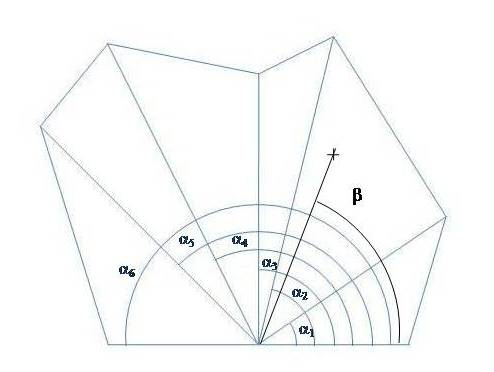
\includegraphics[scale=0.7]{poligono}\\
  \caption{ Ángulos a medir para ver si un punto está dentro de un polígono no convexo}\label{fg:poligono}
\end{figure}


El polígono será, por lo general, no convexo. El algoritmo utilizado para ver si un punto se encuentra en su interior requiere medir los ángulos $\alpha_{1},\alpha_{2},...\alpha_{v}$ indicados en la figura \ref{fg:poligono}. Para cada punto del mapa (tras calcular sus coordenadas en el sistema de referencia local en el láser), se halla el valor del ángulo $\beta$ y se mira entre qué dos alphas está comprendido ($\alpha_{1}$ y $\alpha_{2}$ en el caso de la figura). Con esto se seleccionan dos vértices que servirán para ver si el punto del mapa está dentro del polígono. Se mide la distancia del robot al punto del mapa y se compara con la distancia entre el robot y el vértice de los dos anteriores que sea más cercano al mismo(criterio conservador). Si resulta ser menor, será que el punto se encuentra dentro del polígono.

De este modo, para cada punto del mapa sólo ha de calcularse un ángulo. Esto permite una velocidad de ejecución aceptable.

\section{La clase \prog{CKalman\_ Loc}}
Esta clase se ha creado para gestionar las operaciones relacionadas con el tratamiento de los mapas de puntos que se utilizan y, fundamentalmente, la localización del robot en cada instante. Aparte del constructor, contiene las funciones que se describen brevemente a continuación.

\subsection{KalmanPos}

\prog{void KalmanPos(float inc\_ odom\_x, float inc\_ odom\_ y, float } \prog{inc\_ odom\_ theta)}

En esta función se realizan los cálculos correspondientes a la fase de predicción del algoritmo de localización.

\begin{itemize}
  \item \prog{inc_odom_x}: incremento de odometría medido sobre el eje x del sistema local en el robot
  \item \prog{inc_odom_y}: incremento de odometría medido sobre el eje y del sistema local en el robot
  \item \prog{inc_odom_theta}: variación incremental odométrica en la orientación del robot
\end{itemize}

La posición resultante se almacena en una variable miembro de tipo \prog{Matrix} llamada \prog{pos_robot_kalman}.

\subsection{KalmanUpdate}

\prog{void KalmanUpdate(const std::vector<Point2D>\& v)}

Esta función efectúa la fase de corrección de la localización a partir de la posición obtenida mediante la predicción y de las observaciones que se le pasan.

\begin{itemize}
  \item \prog{v}: vector de la STL que contiene los puntos correspondientes a las observaciones realizadas por el láser
\end{itemize}

El resultado se guarda nuevamente en la variable \prog{pos\_robot\_kalman}.

Inicialmente el mapa (vector de la STL que almacena objetos de la clase Point2D) se encontrará vacío si no se utiliza uno ya realizado. Como ya se ha explicado, las observaciones que no se asocian a ningún punto del mapa se añaden como puntos del mismo si así se selecciona mediante la variable miembro \prog{actualiza} (controlable desde el cuadro de diálogo mediante un \emph{Check box})

%Para los puntos del mapa que no se asocian a una observación, pero se encuentran cercanos a ella o a la mejor estimación de la posición del robot en ese momento,
Para cada uno de los puntos del mapa se comprueba si están en el interior del polígono de observaciones mediante \ref{PuntoEnPol}. En caso afirmativo, y si así lo indica la variable miembro \prog{borrar}, se eliminan del vector \prog{mapa}. Esto es posible porque el polígono es previamente calculado en cada iteración mediante un objeto de la clase \prog{CProcLaserData} perteneciente a la clase \prog{CRobot}. Sus puntos se almacenan en un vector de la STL al cual apunta un puntero miembro de \prog{CKalmanLoc}, \prog{pol}.

\subsection{GuardarMapa}\label{GuardarMapa}

\textbf{void GuardarMapa(LPTSTR path)}

Esta función sirve para guardar un fichero de puntos del mapa de forma que si se dispone de un buen mapa no sea necesario realizar uno nuevo. También resulta útil para examinar los mapas generados o para agilizar algunas pruebas.

\begin{itemize}
  \item path:  \emph{path} en el que guardar un fichero de texto que contendrá dos columnas con las coordenadas de los puntos de un mapa
\end{itemize}

\subsection{LeerMapa}

\prog{void LeerMapa(LPTSTR path)}

Esta función se emplea para descargar un mapa ya creado (por medio de \ref{GuardarMapa}, generalmente).

\begin{itemize}
  \item \prog{path}:  \emph{path} de un fichero de texto ya existente en el que se definen los puntos de un mapa mediante dos columnas de coordenadas
\end{itemize}

A medida que se van leyendo puntos se guardan en el vector \prog{mapa}.

\subsubsection{}
Para que las dos funciones anteriores se ejecuten adecuadamente en Visual Studio .NET 2005 en los \emph{Settings} o \emph{Propiedades} del proyecto no debe marcarse la utilización del juego de caracteres Unicode.

\subsection{PuntoEnPol}\label{PuntoEnPol}

\prog{int PuntoEnPol(int k)}

Esta función sirve para determinar si un punto del mapa se encuentra en el interior del polígono al que apunta el puntero \prog{pol}.

\begin{itemize}
  \item \prog{k}: índice del punto del mapa cuya pertenencia al polígono se quiere determinar
\end{itemize}

Si el punto $k$ del vector \prog{mapa} está en el interior del polígono de observaciones de acuerdo con los criterios establecidos, se devuelve un 1 para que sea eliminado del mapa. En caso contrario la función devuelve un 0.


\section { Otras funciones de la clase \prog{CProcLaserData}}


\subsection {CalculaPol}

\prog{void CalculaPol()}

Esta función se utiliza para crear un polígono envolvente de las observaciones realizadas por el láser.
Inicializa el número de puntos que lo forman a 0 y después hace una llamada a la función recursiva \prog{Split}, que se describe a continuación.

\subsection {Split}

\prog{void Split(int primer, int segun)}

Función recursiva que permite ir obteniendo los segmentos que formarán el polígono con las propiedades mencionadas.

\begin{itemize}
  \item \prog{primer}: índice de la observación a partir de la cual se van a hallar nuevos segmentos
  \item \prog{segun}: índice de la observación hasta la cual se calculan segmentos
\end{itemize}

Se trata de la implementación del proceso descrito al principio de \ref{poligono}.

\vspace{0.2cm}
\noindent
Estas dos funciones no han sido realizadas dentro del proyecto. Se incluyen en este capítulo en lugar de en el anterior para que pueda comprenderse mejor su utilización.

\subsection{ConviertePol}

\prog{void ConviertePol(Matrix pos)}

Esta función calcula las coordenadas de los vértices del polígono en el sistema de referencia global.

\begin{itemize}
  \item \prog{pos}: posición del robot. Se emplea la mejor estimación disponible en cada iteración.
\end{itemize}

Se utiliza principalmente para trazar el dibujo del polígono y para medir distancias de los puntos del mapa a los lados del mismo.
\subsection{PolAng}

\noindent
\prog{void PolAng(Matrix pos)}

Método que se emplea para calcular los ángulos $\alpha$ de la figura \ref{fg:poligono}.

\begin{itemize}
  \item \prog{pos}: posición del robot. Se emplea la mejor estimación disponible en cada iteración.
\end{itemize}

Se aplica un coeficiente de acercamiento de los vértices del polígono al robot y posteriormente se calcula el ángulo $\alpha$ de cada vértice. Estos ángulos se almacenan en un vector \prog{angulos} de la STL variable miembro de la clase.

\section{Pruebas y resultados}
Las pruebas relativas a la localización y a la construcción de mapas de puntos se han efectuado en los modos fichero y real. En simulación las medidas del láser se consideran con alcance constante, por lo que no aportan información que permita la localización.

\subsection{Pruebas en modo \emph{fichero}}
En estas pruebas, se han empleado datos de odometría y del láser obtenidos con diferentes robots y en diferentes entornos por Diego Rodríguez-Losada en el marco de su tesis doctoral. Se ha estudiado el funcionamiento del algoritmo implementado por medio de ficheros que contienen esos datos alternando líneas de tipo representado en la figura \ref{fg:ficheropos} (datos de la odometría) y líneas del tipo representado en la figura \ref{fg:ficherolaser} (datos de medidas del láser). Estas pruebas resultan de mucha utilidad ya que utilizan gran variedad de datos y permiten evaluar el funcionamiento del sistema en entornos muy distintos y con medidas de diferentes características..

\subsubsection{Utilización de datos tomados en el laboratorio de DISAM-UPM}
En este caso, los datos empleados contienen 181 medidas del láser cada vez. Debe recordarse que, por motivos de coste computacional, el algoritmo de localización emplea una de cada dos de ellas. Como estos datos fueron obtenidos con el robot Urbano, no es necesario modificar el \emph{offset} del láser utilizado en el programa.

\noindent
\textbf{\textbf{1.} En esta prueba se han utilizado los siguientes parámetros:}
\begin{itemize}
  \item desviación típica del ruido de la odometría introducida en el filtro de Kalman: $\sigma_{odom} = 0.1$
  \item desviación típica del ruido de las medidas del láser: $\sigma_{med} = 0.3$
  \item ruido adicional: $\sigma_{extra} = 0$
  \item borrado de puntos dinámicos del mapa: $borrar = false$
  \item incorporación de nuevos puntos al mapa: $actualiza = true$
\end{itemize}


\textbf{Resultados:}

En la siguiente figura se puede ver el resultado de la ejecución del programa con las condiciones indicadas. Las sucesivas posiciones del robot según los datos de odometría disponibles serían las representadas en color verde, mientras que la trayectoria corregida mediante el filtro de Kalman es la mostrada en color rojo. Los puntos del mapa creado aparecen en color negro.

\begin{figure}[h]
  % Requires \usepackage{graphicx}
  \centering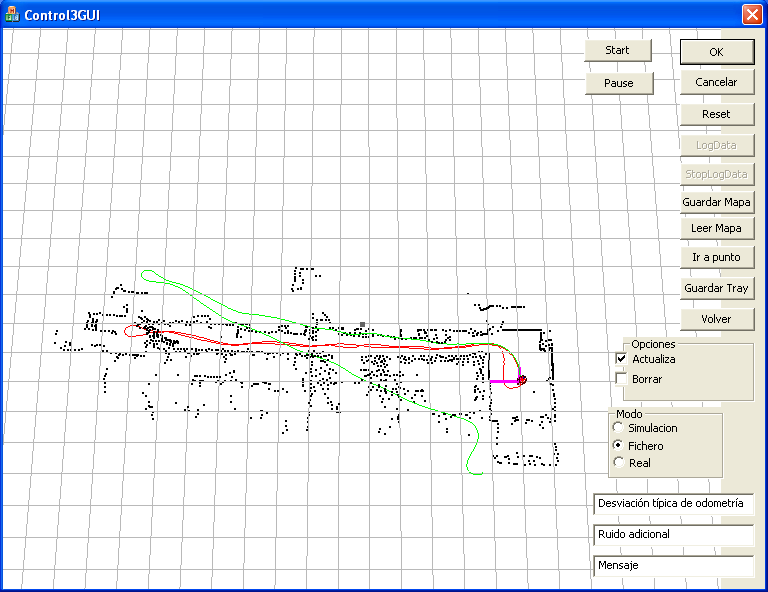
\includegraphics[scale=0.4]{labo1}\\
  \caption{Primer experimento con datos del laboratorio}\label{fg:labo1}
\end{figure}

Se puede apreciar el buen funcionamiento del algoritmo, que permite situar el robot adecuadamente en el mapa y ofrece un valor de posición final muy similar al de la posición de partida del robot.

El tiempo total empleado en la obtención del mapa y en el cálculo de la trayectoria corregida es: 3.54min.

\noindent
\textbf{2.} \textbf{En esta prueba se han utilizado los siguientes parámetros:}
\begin{itemize}
  \item desviación típica del ruido de la odometría introducida en el filtro de Kalman: $\sigma_{odom} = 0.3$
  \item desviación típica del ruido de las medidas del láser: $\sigma_{med} = 0.3$
  \item ruido adicional: $\sigma_{extra} = 0$
  \item borrado de puntos dinámicos del mapa: $borrar = false$
  \item incorporación de nuevos puntos al mapa: $actualiza = true$
\end{itemize}


\textbf{Resultados:}

\begin{figure}[h]
  % Requires \usepackage{graphicx}
  \centering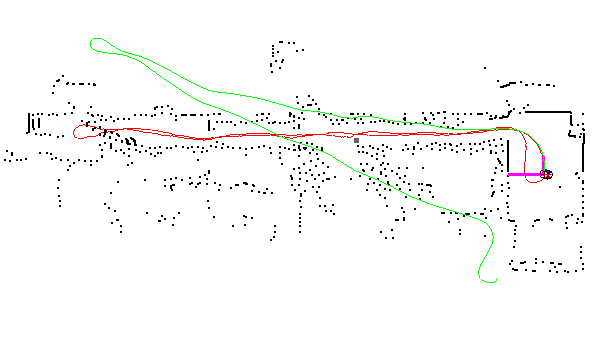
\includegraphics[scale=0.4]{labo2}\\
  \caption{Segundo experimento con datos del laboratorio}\label{fg:labo2}
\end{figure}

Al no ser excesivamente malos los datos de la odometría, no se logran demasiadas mejoras en la localización tras otorgar una mayor importancia a las medidas del láser frente a dichos datos. Sin embargo, puede verse que la parte izquierda del mapa obtenido en este caso es más precisa.

El tiempo total empleado en la obtención del mapa y en el cálculo de la trayectoria es: 3.22min. La disminución del tiempo de ejecución es resultado de la mejor asociación de observaciones a puntos del mapa, que hace que éste tenga un menor tamaño.

\vspace{5cm}
\noindent
\textbf{3.} \textbf{En esta prueba se han utilizado los siguientes parámetros:}
\begin{itemize}
  \item desviación típica del ruido de la odometría introducida en el filtro de Kalman: $\sigma_{odom} = 0.3$
  \item desviación típica del ruido de las medidas del láser: $\sigma_{med} = 0.3$
  \item ruido adicional: $\sigma_{extra} = 0$
  \item borrado de puntos dinámicos del mapa: $borrar = true$
  \item incorporación de nuevos puntos al mapa: $actualiza = true$
\end{itemize}


\textbf{Resultados:}

\begin{figure}[h]
  % Requires \usepackage{graphicx}
  \centering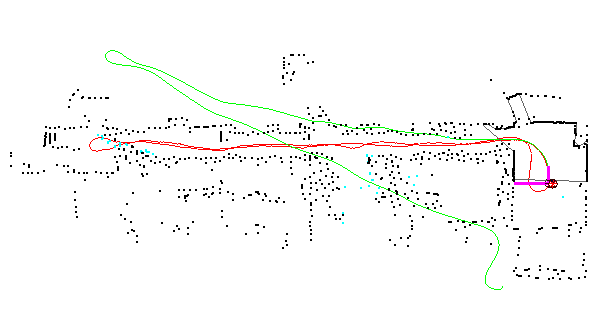
\includegraphics[scale=0.4]{labo3}\\
  \caption{Tercer experimento con datos del laboratorio}\label{fg:labo3}
\end{figure}

Puede verse que cuando se tomaron estos datos había algunas personas moviéndose cerca del recorrido realizado por el robot. Esta opción de ejecución permite borrar del mapa los puntos correspondientes a las posiciones que fueron ocupando (puntos de color cyan en la figura). La localización no resulta afectada de manera significativa por el borrado de dichos puntos. En la figura queda representado el polígono envolvente de las medidas del láser correspondiente a la última posición del robot.

El tiempo total empleado en la obtención del mapa y en el cálculo de la trayectoria corregida es: 3.63min. El cálculo de los puntos del polígono, el de los ángulos necesarios para aplicar el algoritmo de borrado y el análisis de los puntos del mapa no asociados a cada observación en las sucesivas iteraciones( llamadas al método \prog{KalmanUpdate}) provocan un cierto retardo en la ejecución del programa. Este tiempo, no obstante, es considerablemente inferior al correspondiente a otros algoritmos para examinar si un punto pertenece o no a un polígono (algoritmo de Jordan, algoritmo radial\ldots). Además, cada observación nueva ha de compararse con un número menor de puntos del mapa, con lo que en algunos casos el retardo puede quedar prácticamente compensado.

\textbf{4.} \textbf{En esta prueba se han utilizado los siguientes parámetros:}
\begin{itemize}
  \item desviación típica del ruido de la odometría introducida en el filtro de Kalman: $\sigma_{odom} = 0.6$
  \item desviación típica del ruido de las medidas del láser: $\sigma_{med} = 0.3$
  \item ruido adicional: $\sigma_{extra} = 0.005$
  \item borrado de puntos dinámicos del mapa: $borrar = false$
  \item incorporación de nuevos puntos al mapa: $actualiza = true$
\end{itemize}


\textbf{Resultados:}

\begin{figure}[h]
  % Requires \usepackage{graphicx}
  \centering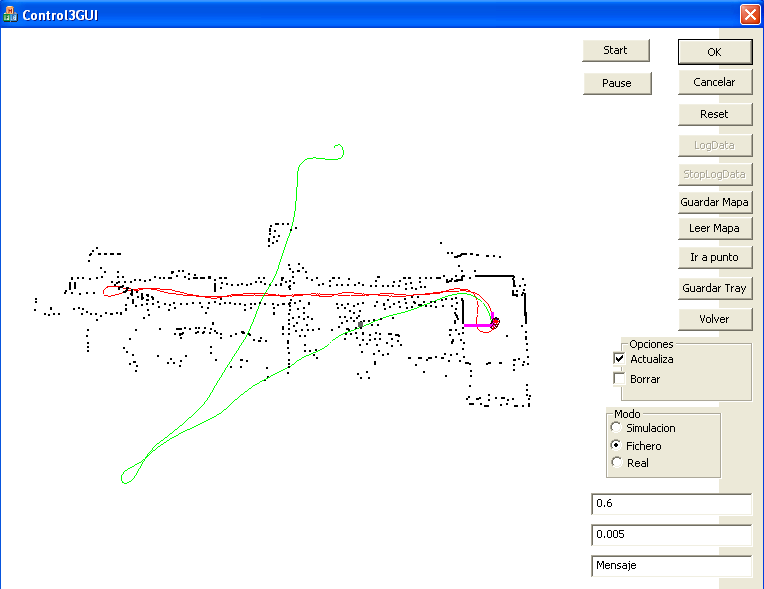
\includegraphics[scale=0.4]{labo4}\\
  \caption{Cuarto experimento con datos del laboratorio}\label{fg:labo4}
\end{figure}

Al inyectarse algo de ruido añadido en las medidas odométricas, la posición del robot estimada en base a dichas medidas está muy alejada de la real. Sin embargo, mediante el algoritmo de localización se sigue obteniendo un buen resultado con sólo volver a incrementar el parámetro considerado en el EKF como varianza del ruido de la odometría.

El tiempo total empleado en la obtención del mapa y en el cálculo de la trayectoria corregida es: 3.15min. Tras tenerse en cuenta que la varianza del ruido de la odometría debe ser algo superior, se mejora la asociación de datos y con ello disminuye el tiempo de procesamiento.


\subsubsection{Utilización de datos de Intel}
Con estos datos, el número de medidas del láser disponibles en cada momento es 361. Esto repercute en el tiempo de procesamiento.

\noindent
\textbf{\textbf{1.} En esta prueba se han utilizado los siguientes parámetros:}
\begin{itemize}
  \item desviación típica del ruido de la odometría introducida en el filtro de Kalman: $\sigma_{odom} = 0.1$
  \item desviación típica del ruido de las medidas del láser: $\sigma_{med} = 0.3$
  \item ruido adicional: $\sigma_{extra} = 0$
  \item borrado de puntos dinámicos del mapa: $borrar = false$
  \item incorporación de nuevos puntos al mapa: $actualiza = true$
\end{itemize}


\textbf{Resultados:}


\begin{figure}[h]
  % Requires \usepackage{graphicx}
  \centering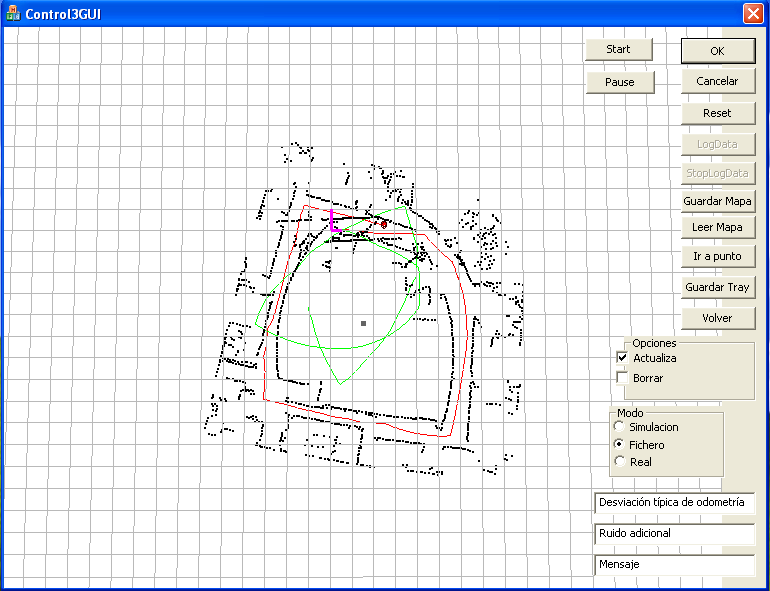
\includegraphics[scale=0.4]{intel1}\\
  \caption{Primer experimento con datos de Intel}\label{fg:intel1}
\end{figure}

Se puede observar que las medidas odométricas presentan un alto grado de error. Por ello, es muy probable que la varianza introducida en el filtro de Kalman para dichas medidas sea demasiado pequeña y, por lo tanto, la elaboración del mapa no sea la correcta.

El tiempo total empleado en la obtención del mapa y en el cálculo de la trayectoria corregida es: 6.8min.

\vspace{5cm}
\noindent
\textbf{2.} \textbf{En esta prueba se han utilizado los siguientes parámetros:}
\begin{itemize}
  \item desviación típica del ruido de la odometría introducida en el filtro de Kalman: $\sigma_{odom} = 0.8$
  \item desviación típica del ruido de las medidas del láser: $\sigma_{med} = 0.3$
  \item ruido adicional: $\sigma_{extra} = 0$
  \item borrado de puntos dinámicos del mapa: $borrar = false$
  \item incorporación de nuevos puntos al mapa: $actualiza = true$
\end{itemize}


\textbf{Resultados:}

\begin{figure}[h]
  % Requires \usepackage{graphicx}
  \centering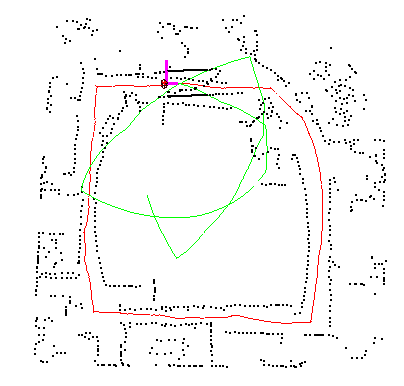
\includegraphics[scale=0.4]{intel2}\\
  \caption{Segundo experimento con datos de Intel}\label{fg:intel2}
\end{figure}

En este caso, la varianza del ruido de las medidas de odometría estimada para la utilización del filtro de Kalman resulta más adecuada y, como puede observarse, conduce a un resultado excelente a pesar de la poca calidad de los datos odométricos disponibles.

El tiempo total empleado en la obtención del mapa y en el cálculo de la trayectoria corregida es: 5.71min.

%\vspace{0.4cm}
%\vspace{0.4cm}
\noindent
\textbf{3.} \textbf{En esta prueba se han utilizado los siguientes parámetros:}
\begin{itemize}
  \item desviación típica del ruido de la odometría introducida en el filtro de Kalman: $\sigma_{odom} = 1$
  \item desviación típica del ruido de las medidas del láser: $\sigma_{med} = 0.3$
  \item ruido adicional: $\sigma_{extra} = 0$
  \item borrado de puntos dinámicos del mapa: $borrar = true$
  \item incorporación de nuevos puntos al mapa: $actualiza = true$
\end{itemize}


\textbf{Resultados:}

\begin{figure}[h]
  % Requires \usepackage{graphicx}
  \centering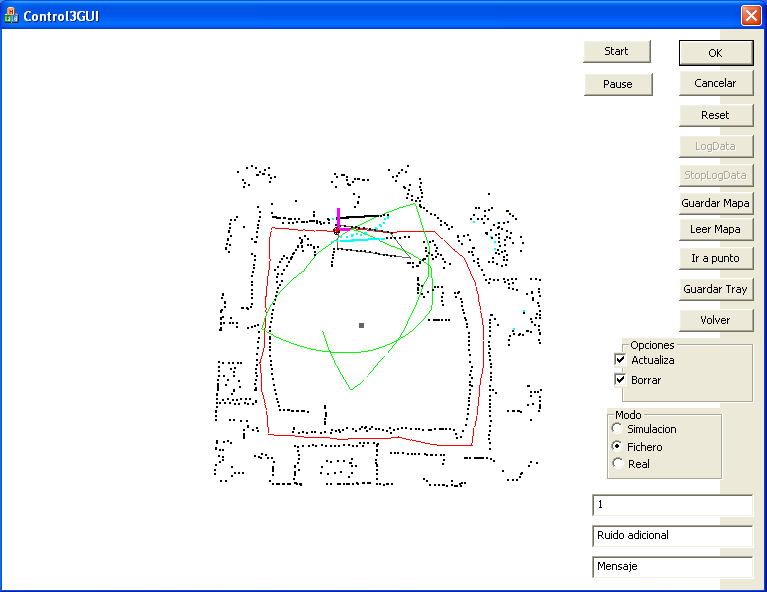
\includegraphics[scale=0.4]{intel3}\\
  \caption{Tercer experimento con datos de Intel}\label{fg:intel3}
\end{figure}

El tiempo total empleado en la obtención del mapa y en el cálculo de la trayectoria corregida es: 6.61min.

\subsubsection{Utilización de datos del Museo de las Ciencias Príncipe Felipe de Valencia}
Estos datos incluyen 181 medidas del láser en cada momento. Por esta razón su procesamiento resulta más ágil que el del caso anterior. No obstante, dada la gran extensión del mapa elaborado y la exhaustiva exploración del entorno para la realización del mismo, el tiempo total consumido es notablemente superior por serlo también la duración del recorrido de toma de datos.

\noindent
\textbf{\textbf{1.} En esta prueba se han utilizado los siguientes parámetros:}
\begin{itemize}
  \item desviación típica del ruido de la odometría introducida en el filtro de Kalman: $\sigma_{odom} = 0.9$
  \item desviación típica del ruido de las medidas del láser: $\sigma_{med} = 0.3$
  \item ruido adicional: $\sigma_{extra} = 0$
  \item borrado de puntos dinámicos del mapa: $borrar = false$
  \item incorporación de nuevos puntos al mapa: $actualiza = true$
\end{itemize}


\textbf{Resultados:}
\begin{figure}[h]
  % Requires \usepackage{graphicx}
  \centering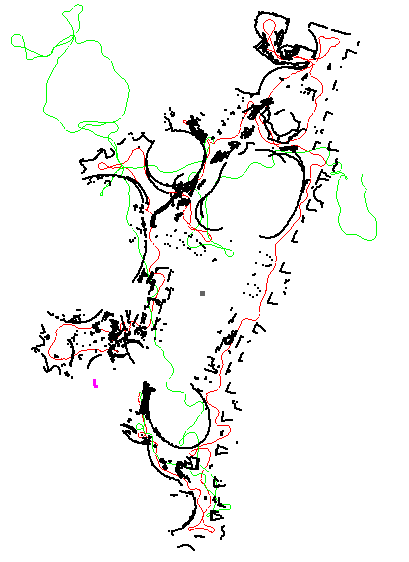
\includegraphics[scale=0.4]{val3}\\
  \caption{Primer experimento con datos del Museo de las Ciencias Príncipe Felipe de Valencia}\label{fg:val3}
\end{figure}

El tiempo total empleado en la obtención del mapa y en el cálculo de la trayectoria corregida es: 26.54min.


\noindent
\textbf{\textbf{2.} En esta prueba se han utilizado los siguientes parámetros:}
\begin{itemize}
  \item desviación típica del ruido de la odometría introducida en el filtro de Kalman: $\sigma_{odom} = 0.9$
  \item desviación típica del ruido de las medidas del láser: $\sigma_{med} = 0.3$
  \item ruido adicional: $\sigma_{extra} = 0$
  \item borrado de puntos dinámicos del mapa: $borrar = true$
  \item incorporación de nuevos puntos al mapa: $actualiza = true$
\end{itemize}


\textbf{Resultados:}
\begin{figure}[h]
  % Requires \usepackage{graphicx}
  \centering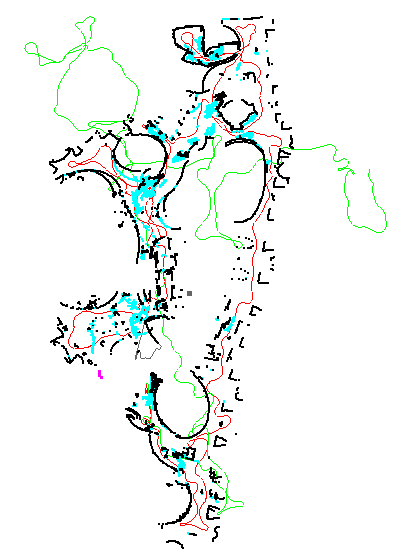
\includegraphics[scale=0.4]{val2}\\
  \caption{Segundo experimento con datos del Museo de las Ciencias Príncipe Felipe de Valencia}\label{fg:val2}
\end{figure}

El tiempo total empleado en la obtención del mapa y en el cálculo de la trayectoria corregida es: 36.01min.

\vspace{0.2cm}
\noindent
Como puede observarse, la presencia de personas en el museo afecta a la construcción del mapa y a la localización. Esto puede corregirse mediante el borrado de puntos del mapa, con lo que se logra un resultado realmente bueno. A pesar de la gran longitud de la trayectoria seguida, con el correspondiente incremento de errores en las medidas de los encoders, el sistema mantiene una correcta estimación de la posición del robot hasta el final del recorrido efectuado.



